By profiling the preprocessing pipelines, we aim to provide insights about how to pick the optimal preprocessing strategy for a specific set of hardware, the datasets, and the characteristics of each pipeline.
The goal is to maximize the $T_4$ throughput (Fig.~\ref{fig:generic-dl-pipeline}) while keeping the storage consumption and offline preprocessing time low.
Our analysis is focused on four core aspects:
\begin{description}[align=left]
    \item[Storage Consumption versus Throughput:] 

    {\color{diff}A high storage consumption can render extensive offline preprocessing useless or even counterproductive to achieve high throughput.
    This has two causes. First, the dataset may be split into many files, and the storage does not respond fast enough to random read access, leading to a storage bottleneck.
    Secondly, specific preprocessing steps (e.g., normalizing an integer range to floating points) inflate the data volume.
    This can lead to a lower throughput because the saved preprocessing time is outweighed by the increased data ingestion time (see Section~\ref{ssec:storage-versus-throughput}).}

    \item[Caching:]

    {\color{diff}As a DL training process typically iterates over the dataset multiple times, there can be an increased throughput due to caching effects after the first epoch.
    However, this effect depends on whether the preprocessed training data fits into memory.
    Further, reading the cached dataset from memory can help to isolate processing bottlenecks from storage bottlenecks (see Section~\ref{ssec:caching}).}

    \item[Compression:]

    {\color{diff}Compression provides a way to trade off CPU overhead for en-/decode steps against smaller storage consumption.
    We profile each strategy with GZIP~\cite{10.17487/RFC1952} and ZLIB~\cite{10.17487/RFC1950} compression and show under which circumstances compression improves the throughput (see Section~\ref{ssec:compression}).}

    % \item[{\color{diff}Number of Samples:}]

    % Profiling takes time, which may be too costly depending on the dataset.
    % We compare the generated profiles based on small samples of each dataset to the entire dataset, which provides information about how well the insights can be extrapolated.
    % We discuss these findings in Section~\ref{ssec:extrapolation-sampling}.

    \item[Parallelization Capabilities:]
    Preprocessing steps can hinder performance if multi-core CPUs are not utilized effectively.
    Scalability bottlenecks may have a substantial impact on throughput.
    We compare the speedup of each preprocessing step under multi-threading and {\color{diff}system-level caching} in Section~\ref{ssec:parallelization-capabilities}.

\end{description}
We also touch on shuffling (see Section~\ref{ssec:shuffling}) {\color{diff}and discuss how to introduce new steps to an already profiled CV pipeline based on a case study in Section~\ref{ssec:modifying-pipeline}.}
\vspace{-0.25cm}
\begin{table}[h]
\scalebox{0.8}{
\begin{tabular}{r|r|r|r|r}
\textbf{Threads} & \textbf{Files per Thread} & \textbf{Bandwidth} & \textbf{Latency} & \textbf{IOPS} \\ \hline
 1 & 1 & 219\:MB/s & $4-10\mu\text{s}$ &  53400 \\
 8 & 1 & \textbf{910\:MB/s} & $4-10\mu\text{s}$ & \textbf{222000} \\ \hline
 1 & 5000 & 6.6\:MB/s & $4-10\mu\text{s}$ & 1629 \\
 8 & 5000 & 40.4\:MB/s & $4-10\mu\text{s}$ & 9853 
\end{tabular}
}
\caption{{\color{diff}\texttt{fio} profile of our storage cluster}}
\label{tab:storage-bw}
\end{table}
\vspace{-0.9cm}

\subsection{Storage Consumption versus Throughput}
\label{ssec:storage-versus-throughput}

We profiled the throughput and storage consumption for all strategies of each pipeline in Figure~\ref{fig:ss-vs-thr}.
{\color{diff}The theoretical network read speed to the HDD-backed Ceph storage cluster is capped at 1.25\:GB/s (10\:Gb/s) due to hardware limitations, but the actual rates differ based on the access pattern.
To provide a pipeline-independent measurement, we profiled four workloads with the \texttt{fio} tool~\cite{fio} to simulate both sequential and random file access with 5000 files of 0.2\:MB each and with one 5\:GB file, which is comparable to our \texttt{unprocessed} and \texttt{concatenated} strategies.
Additionally, we tested the single-threaded performance compared to 8 threads with the same workload per thread.
Table~\ref{tab:storage-bw} shows that reading sequentially is 33$\times$ faster for single- and 22$\times$ faster for multi-threaded execution.
While our single-threaded bandwidth is limited to 219\:MB/s, the multi-threaded execution is close to the hardware cap with 910\:MB/s.
This helps to explain our main observations:}

{\color{diff}
\vspace{-0.2cm}
\begin{table}[h]
\scalebox{0.8}{
\begin{tabular}{l|r|r|r|r}
\textbf{Pipeline} & \multicolumn{2}{c|}{\textbf{Throughput in SPS}} & \multicolumn{2}{c}{\textbf{Network Reads in MB/s}}  \\ \hline
                  & \texttt{unprocessed} & \texttt{concatenated} & \texttt{unprocessed} & \texttt{concatenated}  \\ \hline
CV                & 107 & \textbf{962} & ($\pm 3$) 12 & ($\pm 16$) \textbf{111} \\ \hline
CV (SSD)          & 588 & \textbf{944} & ($\pm 8$) 68 &    ($\pm 15$) \textbf{108} \\ \hline
CV2-JPG           & 88  & \textbf{288} & ($\pm 11$) 46 &    ($\pm 72$) \textbf{110}  \\ \hline
CV2-PNG           & 15  & \textbf{21}  & ($\pm 37$) 270 &   ($\pm 54$) \textbf{390}  \\ \hline
NLP               & 6   & 6   & ($\pm 0.2$) 0.21 &  ($\pm 1.5$) \textbf{0.26}  \\ \hline
NLP (SSD)         & 3   & 3   & ($\pm 0.2$) \textbf{0.17} &  ($\pm 1.2$) 0.16  \\
\end{tabular}
}
\caption{{\color{diff}Throughput and average network read speeds for strategies with concatenation.}}
\label{tab:concatenated-throughput-reads}
\end{table}
\vspace{-0.7cm}

\textbf{(1) Concatenating can increase throughput significantly.}

An I/O bottleneck may arise when the storage cannot saturate the hardware bandwidth based on the data access pattern.
Out of the four pipelines which have a \texttt{concatenated} strategy (CV, CV2-JPG, CV2-PNG, and NLP), we see that all CV-based pipelines have a throughput increase between 1.4$\times$ and 9$\times$ compared to the \texttt{unprocessed} strategy (Table~\ref{tab:concatenated-throughput-reads}).
The individual differences in the throughput can be explained by the dataset size and the average storage consumption of a sample (Table~\ref{tab:experiments:dataset-info}).
Due to the CV samples being smaller than the CV2-JPG samples, CV achieves 962\:SPS compared to 288\:SPS while having a similar network read speed of approximately 110\:MB/s.
The CV2-PNG dataset has a sample storage consumption of 17.4\:MB and the network read speed increases from 270\:MB/s to 390\:MB/s with concatenation.

Contrary to CV-based pipelines, the NLP pipeline does not benefit from concatenating as the throughput stays at 6\:SPS, indicating a CPU bottleneck.
This bottleneck is resolved in the \texttt{decoded} strategy, where throughput increases significantly (Fig.~\ref{fig:ss-vs-thr-nlp}).

As an HDD-based storage solution is particularly vulnerable to random access bottlenecks, we additionally profiled the performance of the CV and NLP pipeline on an SSD-backed Ceph cluster.
The CV \texttt{unprocessed} strategy had a throughput of 588\:SPS, which is almost $6\times$ faster than the HDD experiments.
However, at the \texttt{concatenated} strategy, both HDD and SSD reach roughly the same throughput (962\:SPS vs. 944\:SPS), i.e., at sequential access the SSD-backed storage is not faster.
For NLP, the SSD storage did not provide a better throughput as it still faces the CPU bottleneck at the \texttt{concatenated} strategy.

\vspace{-0.1cm}
\begin{figure}[h]
    \begin{subfigure}[c]{0.22\textwidth}
        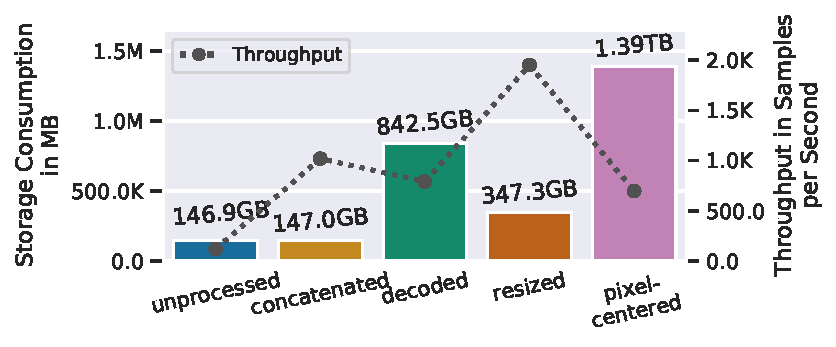
\includegraphics[width=\textwidth]{figures/imagenet-pipeline/storage-vs-throughput.pdf}
        \vspace{-18pt}
        \caption{CV}
        \label{fig:ss-vs-thr-cv}
    \end{subfigure}
    \begin{subfigure}[c]{0.22\textwidth}
        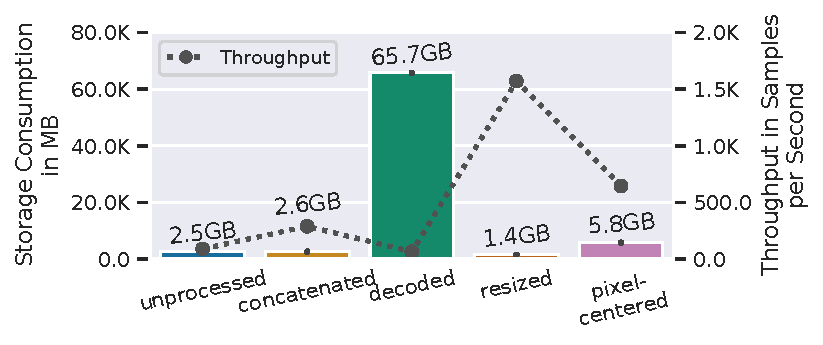
\includegraphics[width=\textwidth]{figures/cubeplusplus-jpg-pipeline/storage-vs-throughput.pdf}
        \vspace{-18pt}
        \caption{CV2-JPG}
        \label{fig:ss-vs-thr-cv2-jpg}
    \end{subfigure}
    \begin{subfigure}[c]{0.22\textwidth}
        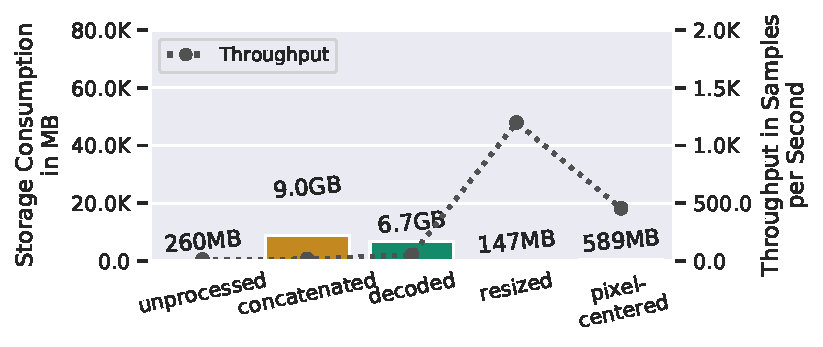
\includegraphics[width=\textwidth]{figures/cubeplusplus-png-pipeline/storage-vs-throughput.pdf}
        \vspace{-18pt}
        \caption{CV2-PNG}
        \label{fig:ss-vs-thr-cv2-png}
    \end{subfigure}
    \begin{subfigure}[c]{0.22\textwidth}
        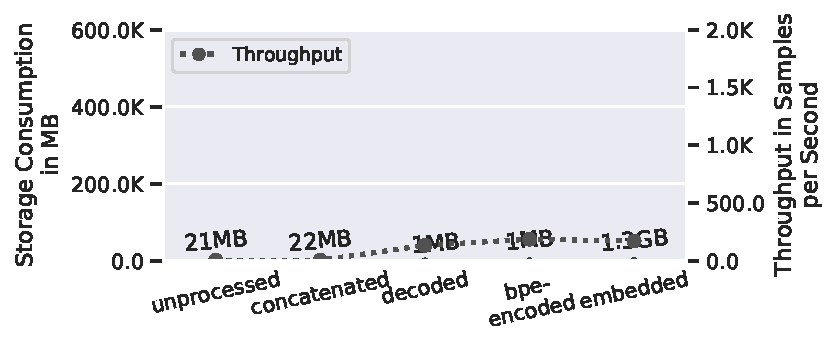
\includegraphics[width=\textwidth]{figures/openwebtext-pipeline/storage-vs-throughput.pdf}
        \vspace{-18pt}
        \caption{NLP}
        \label{fig:ss-vs-thr-nlp}
    \end{subfigure}
    \begin{subfigure}[c]{0.22\textwidth}
        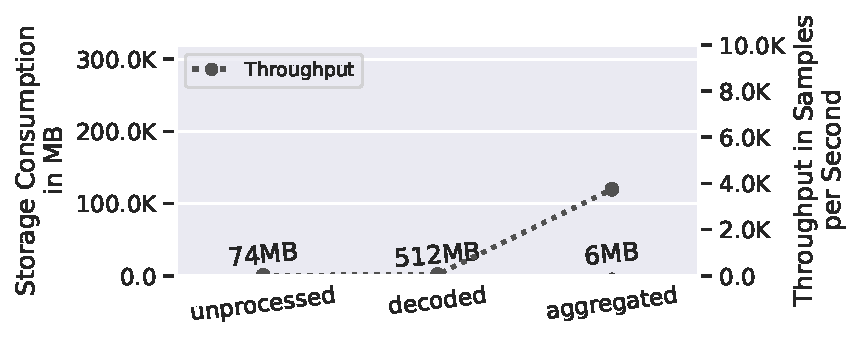
\includegraphics[width=\textwidth]{figures/cream-pipeline/storage-vs-throughput.pdf}
        \vspace{-18pt}
        \caption{NILM}
        \label{fig:ss-vs-thr-nilm}
    \end{subfigure}
    \begin{subfigure}[c]{0.22\textwidth}
        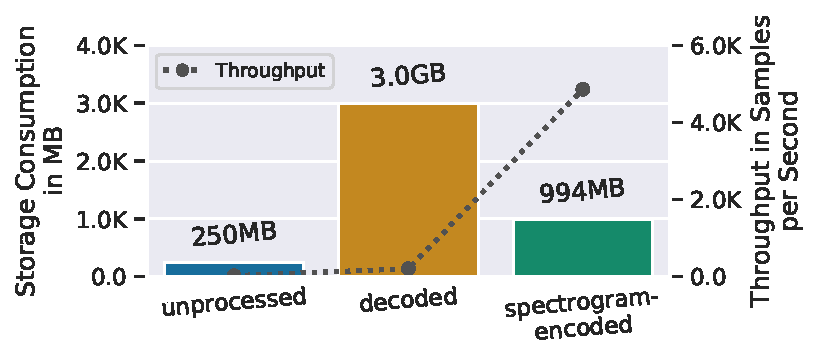
\includegraphics[width=\textwidth]{figures/commonvoice-pipeline/storage-vs-throughput.pdf}
        \vspace{-18pt}
        \caption{MP3}
        \label{fig:ss-vs-thr-mp3}
    \end{subfigure}
    \begin{minipage}[c]{0.22\textwidth}
        \begin{subfigure}[c]{\textwidth}
            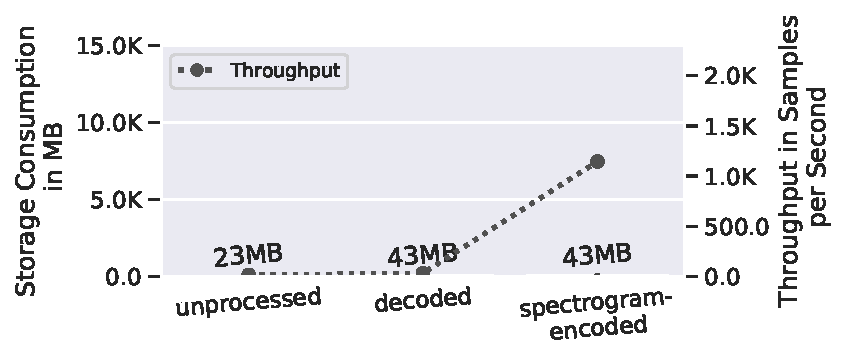
\includegraphics[width=\textwidth]{figures/librispeech-pipeline/storage-vs-throughput.pdf}
            \vspace{-18pt}
            \caption{FLAC}
            \label{fig:ss-vs-thr-flac}
        \end{subfigure}
    \end{minipage}\hspace{5mm}
    \begin{minipage}[c]{0.20\textwidth}
        \vspace{-10pt}
        \caption{Storage consumption (left y-axis) for each dataset representation compared to the $T_4$ throughput (dotted line, right y-axis).}
        \label{fig:ss-vs-thr}
    \end{minipage}
\end{figure}
%\vspace{-0.1cm}

\textbf{(2) The maximum throughput of a strategy is influenced by its storage consumption. }

When the CPU performance in combination with a storage setup can saturate the hardware bandwidth (i.e., in our case, read data with 1.25\:GB/s), then a maximum theoretical throughput can be calculated by dividing the \textit{bandwidth} by the \textit{storage consumption per sample}.
This theoretical throughput is based on two steps.
First, one reads a sample from the storage into memory.
Second, one applies the online transformation steps in succession until the sample can be fed into the training process.
The total time of these two steps defines the pipeline's throughput (i.e., samples per second), hence also the network read speed (i.e., MB per second).
In our case, the actual throughput we can achieve is bound by the multi-threaded read performance to our cluster, which is at 910MB/s with eight threads (Table~\ref{tab:storage-bw}).
This profiled network read speed provides a baseline of the maximum possible throughput.
The goal of every strategy should be to have a short enough transformation step to achieve this baseline read speed.
In turn, if transformation steps are too long, such that the maximum read cannot be reached, we can assume a CPU bottleneck.

A characteristic result of how storage consumption affects the throughput of strategies can be seen in the CV, CV2-JPG, CV2-PNG and NLP pipelines (Fig.~\ref{fig:ss-vs-thr-cv}, \ref{fig:ss-vs-thr-cv2-jpg}, \ref{fig:ss-vs-thr-cv2-png}, \ref{fig:ss-vs-thr-nlp}), where the last strategy has the least amount of online processing to do, but performs worse than its corresponding preceding strategy.
An excellent example of this is the CV pipeline.
At the last strategy, \texttt{pixel-centered}, we have an average network read speed of 585\:MB/s and need to read 1.4\:TB of data.
This stands in contrast to the previous strategy, \texttt{resized}, which has a lower network read speed of 470\:MB/s, but only needs to read 347\:GB.
Therefore, the \texttt{resized} strategy has a more than $3\times$ greater throughput of 1789\:SPS compared to \texttt{pixel-centered} (576\:SPS), even though \texttt{resized} applies more processing steps online.
%As we are not close to our maximum profiled network read speed, both of these strategies suffer from a CPU bottleneck.
%The biggest impact on the throughput was the change of storage consumption, because \texttt{pixel-centered} converts each pixel from a \texttt{uint8} to a \texttt{float32} which effectively quadruples the storage consumption.
The cause of the increased storage consumption is that \texttt{pixel-centered} converts each pixel from an \texttt{uint8} to a \texttt{float32} which effectively quadruples the storage consumption.
All our CV-based pipelines share this characteristic at different magnitudes, which results in the \texttt{resized} strategy having the best throughput.

}


{\color{diff2}
The NLP pipeline has a similar issue with the embedded step, which slows down the throughput from 1726\:SPS with \texttt{bpe-encoded} to 131\:SPS with \texttt{embedded} (a factor of $13\times$).
Applying the embedding step online is very computationally intensive, which yields a data ingestion of only 6\:MB/s for \texttt{bpe-encoded}.
One could think that preprocessing this step offline should improve performance.
But this is not the case, because the storage consumption increases from 647\:MB to 491\:GB, such that the benefit of processing the embedding step offline is outweighed by the increased time to read the dataset.
}

{\color{diff}
The remaining pipelines, NILM, MP3 and FLAC (Fig.~\ref{fig:ss-vs-thr-nilm},~\ref{fig:ss-vs-thr-mp3},~\ref{fig:ss-vs-thr-flac}), share the common characteristic that the last preprocessing step is the most computationally expensive one, which leads to the best throughput when processed offline.
While they all have different storage consumption, none of the pipelines approaches the maximum possible network read speeds at their respective last strategy.

On first sight, this is counter intuitive.
In the last strategy, there is almost no processing to be done except for decoding the read data.
Why do these strategies not approach the network read limit?
A deeper investigation leads to our following observation.

\vspace{-0.47cm}
\begin{figure}[h]
    \centering
    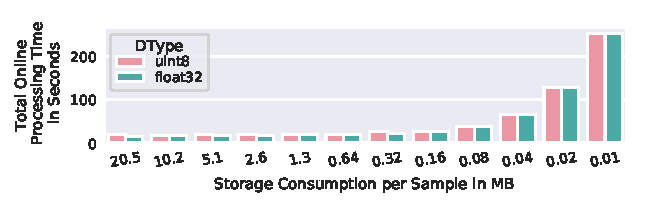
\includegraphics[width=0.47\textwidth]{figures/misc/artificial-dataset}
    \vspace{-14pt}
    \caption{{\color{diff}Profiling a synthetic 15\:GB dataset with different datatypes and sample sizes.}}
    \label{fig:synthetic-dataset}
\end{figure}
\vspace{-0.3cm}

\textbf{(3) A high storage consumption per sample allows for easier I/O bandwidth saturation.}

A deserialization step is applied onto every sample which is read from the storage to transform it from a bytestream into a tensor.
We observed that an increasing sample size positively influences the I/O bandwidth of reading and deserializing.
To provide a basis to our observation, we conduct an experiment with synthetic data that shows the effect of different sample sizes on the online processing time of reading and deserializing.
We evaluate sample sizes from 0.01\:MB to 20.5\:MB with doubling increments while keeping a total storage consumption of 15\:GB for both \texttt{uint8} and \texttt{float32} datatypes which are common in our real-world pipelines.
}
{\color{diff3}
To keep the same total storage consumption with different sample sizes we adapted the sample count, which ranged from 732 (20.5\:MB) to 1.5M (0.01\:MB) samples.
}
{\color{diff}
Figure~\ref{fig:synthetic-dataset} shows the result that reading the same amount of data with different sample sizes has a major effect on the processing time.
A dataset consisting of large (20.5\:MB) samples takes less than half the processing time of small ($\leq0.08$\:MB) samples.
At a sample size of 0.01\:MB, it takes more than $11\times$ longer to process the 15\:GB of data compared to 20.5\:MB samples.
Finally, the different data types do not have an impact on the processing time, as both \texttt{uint8} and \texttt{float32} show similar results.

% Initially, it seems that allowing faster read performance would benefit the $T_4$ throughput, which stands in contrast to the observation \textbf{(2)}, whereas a high storage consumption affects the throughput negatively.
% However, this is not the case in our experiments.
A good example for this observation is the comparison of the \texttt{decoded} strategy between CV (Fig.~\ref{fig:ss-vs-thr-cv}) and CV2-JPG (Fig.~\ref{fig:ss-vs-thr-cv2-jpg}).
%The CV2-JPG \texttt{decoded} strategy has a throughput of 64\:SPS, which is lower than the \texttt{concatenated} strategy with 288\:SPS.
%As the storage consumption jumps to its highest point at 65.7\:GB, the preprocessing has to read $25\times$ more data, leading to the slowdown.
The average sample size is 13\:MB for the \texttt{decoded} strategy of CV2-JPG with a network read speed of 828\:MB/s, which indicates an I/O bottleneck.
%However, we measure an average 828\:MB/s network read speed close to our profiled maximum bandwidth, which indicates an I/O bottleneck.
However, with the same strategy, the CV pipeline has a sample size of 0.6\:MB and the average network read rate is at 491\:MB/s, which is not even close to our maximum bandwidth.
Notably, the CV pipeline has a lower computational load compared to CV2-JPG \textit{and} has to read fewer data from storage with each sample due to the small sample size.
But it still does not manage to saturate the I/O bandwidth.
Therefore, the CV \texttt{decoded} strategy suffers from a CPU bottleneck.
To further validate our assumption, we profiled the CV pipeline with 16 threads which increased the network read speed by 64\:MB/s and improved the throughput by 142\:SPS.
The additional multi-threading also increased the throughput by 583\:SPS and 100\:SPS for the \texttt{resized} and \texttt{pixel-centered}, respectively.
All last strategies like \texttt{aggregated} (Fig.~\ref{fig:ss-vs-thr-nilm}), \texttt{spectrogram-encoded} (Fig.~\ref{fig:ss-vs-thr-mp3},~\ref{fig:ss-vs-thr-flac}), and \texttt{embedded} (Fig.~\ref{fig:ss-vs-thr-nlp}) share that characteristic and do not saturate the I/O bandwidth (96\:MB/s, 317\:MB/s, 564\:MB/s and 315\:MB/s respectively).

}

{\color{diff}
\vspace{-0.3cm}
\subsection{Caching}
\label{ssec:caching}

DL training jobs typically run over multiple epochs, which means the dataset is read multiple times and could benefit from being cached in memory after the first epoch.
We evaluated the throughput of all pipelines over two epochs for all strategies.
In this set of experiments, we do not flush the page cache after the first epoch.
Our observations are as follows:

\textbf{(1) Caching is not beneficial when the storage consumption is higher than the available memory.}

If the data set is too large for the memory, the dataset is read completely from the storage at every epoch.
Hence, throughput is not increased by caching.
All strategies that have a storage consumption higher than 80\:GB (Fig.~\ref{fig:ss-vs-thr}) have the same throughput over all epochs (Fig.~\ref{fig:caching}).

\textbf{(2) Caching does not remove CPU bottlenecks. }

Assuming that the dataset fits into memory, caching can only improve throughput significantly if there is no CPU bottleneck.
Reading data from memory is much faster than from remote network storage, but the impact of fast data access can become insignificant when followed by computationally expensive preprocessing steps.
An excellent example of this is the NLP pipeline (Fig.~\ref{fig:caching-nlp}).
The first two strategies \texttt{unprocessed} and \texttt{concatenated} have the same throughput of 6\:SPS over all epochs because decoding is very compute intensive while the datasize is relatively small (7.7\:GB).
Then, after decoding the data (594\:MB), we face a new computationally expensive step, byte-pair encoding, which transforms the text into integers and increases the storage consumption to 647\:MB.
This is followed by the embedding step, which also takes much time.
All of these strategies face a CPU bottleneck while having a storage consumption that allows the data to be cached.
Finally, at the \texttt{embedded} strategy, the dataset only needs to be read from the storage, but grows in size to 490.7\:GB, such that caching has no impact on throughput.

Similar CPU bottlenecks can also be observed in the \texttt{unprocessed} strategies of CV2-PNG, NILM, MP3 and FLAC (Fig.~\ref{fig:caching-cv2-png},~\ref{fig:caching-nilm},~\ref{fig:caching-mp3},~\ref{fig:caching-flac}), the \texttt{concatenated} strategies of CV2-\{JPG,PNG\} (Fig.~\ref{fig:caching-cv2-jpg},~\ref{fig:caching-cv2-png}) and the \texttt{decoded} strategies of MP3 and FLAC.
The remaining strategies (\texttt{resized}, \texttt{pixel-centered}, \texttt{aggregated}, \texttt{spectrogram-encoded}) benefit from caching the most as they have low storage consumption and are not followed by computationally expensive steps.
However, caching improves the throughput with differing factors ($1.1\times$-$4.2\times$), which results in the next observation.

%\vspace{-0.3cm}
\begin{figure}[h]
    \begin{subfigure}[c]{0.22\textwidth}
        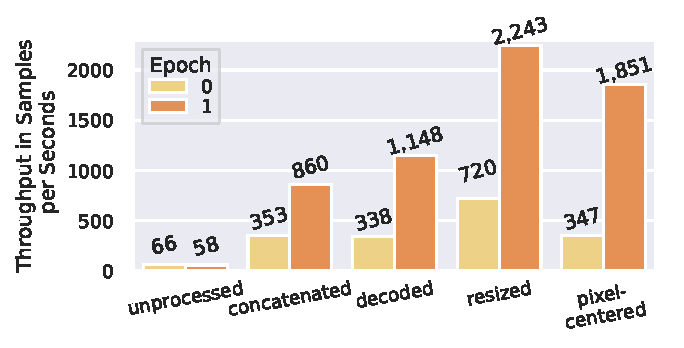
\includegraphics[width=\textwidth]{figures/imagenet-pipeline/caching-over-epochs.pdf}
        \vspace{-18pt}
        \caption{CV}
        \label{fig:caching-cv}
    \end{subfigure}
    \begin{subfigure}[c]{0.22\textwidth}
        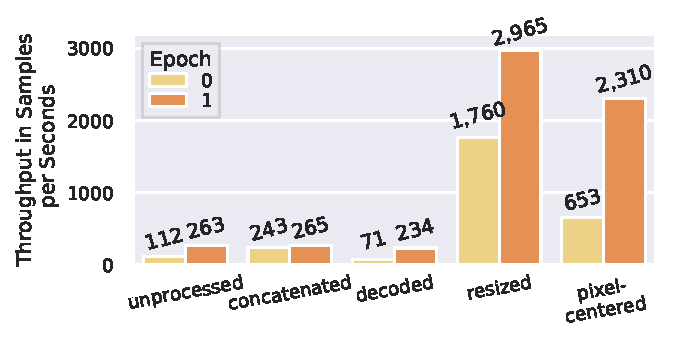
\includegraphics[width=\textwidth]{figures/cubeplusplus-jpg-pipeline/caching-over-epochs.pdf}
        \vspace{-18pt}
        \caption{CV2-JPG}
        \label{fig:caching-cv2-jpg}
    \end{subfigure}
    \begin{subfigure}[c]{0.22\textwidth}
        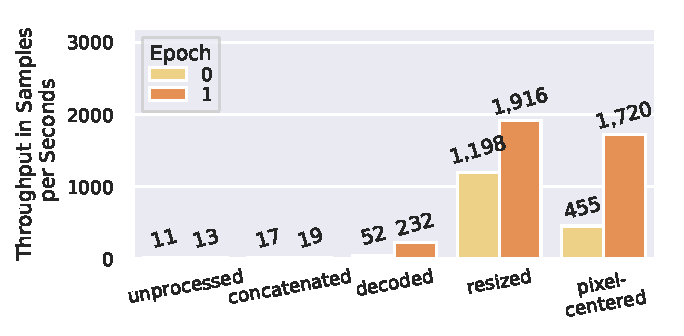
\includegraphics[width=\textwidth]{figures/cubeplusplus-png-pipeline/caching-over-epochs.pdf}
        \vspace{-18pt}
        \caption{CV2-PNG}
        \label{fig:caching-cv2-png}
    \end{subfigure}
    \begin{subfigure}[c]{0.22\textwidth}
        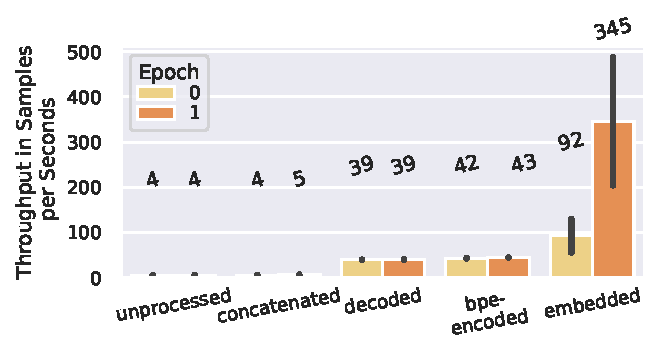
\includegraphics[width=\textwidth]{figures/openwebtext-pipeline/caching-over-epochs.pdf}
        \vspace{-18pt}
        \caption{NLP}
        \label{fig:caching-nlp}
    \end{subfigure}
    \begin{subfigure}[c]{0.22\textwidth}
        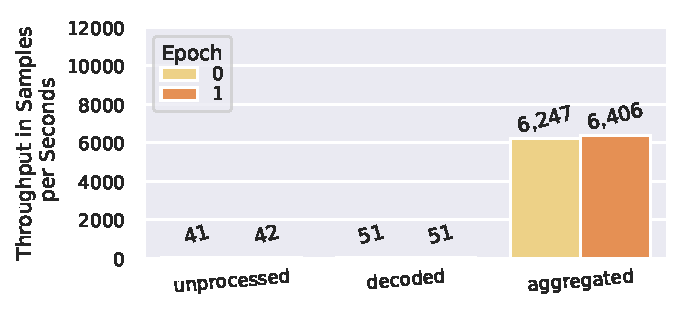
\includegraphics[width=\textwidth]{figures/cream-pipeline/caching-over-epochs.pdf}
        \vspace{-18pt}
        \caption{NILM}
        \label{fig:caching-nilm}
    \end{subfigure}
    \begin{subfigure}[c]{0.22\textwidth}
        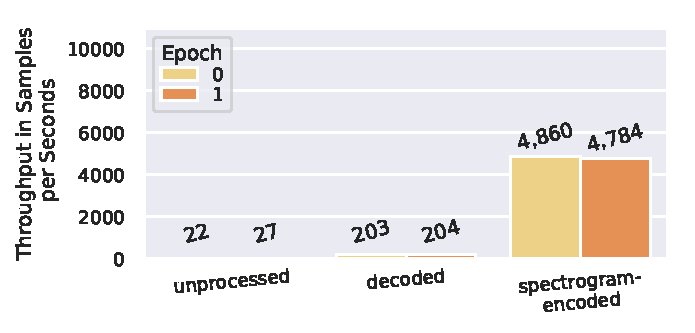
\includegraphics[width=\textwidth]{figures/commonvoice-pipeline/caching-over-epochs.pdf}
        \vspace{-18pt}
        \caption{MP3}
        \label{fig:caching-mp3}
    \end{subfigure}
    \begin{minipage}[c]{0.22\textwidth}
        \begin{subfigure}[c]{\textwidth}
            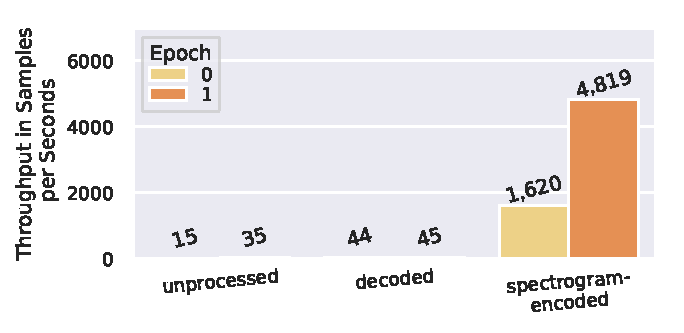
\includegraphics[width=\textwidth]{figures/librispeech-pipeline/caching-over-epochs.pdf}
            \vspace{-18pt}
            \caption{FLAC}
            \label{fig:caching-flac}
        \end{subfigure}
    \end{minipage}\hspace{5mm}
    \begin{minipage}[c]{0.20\textwidth}
        \vspace{-18pt}
        \caption{{\color{diff}Effects of caching on $T_4$ throughput for all pipelines.}}
        \label{fig:caching}
    \end{minipage}
\end{figure}
\vspace{-0.3cm}

\textbf{(3) System-level caching performance is affected by the storage consumption per sample. }

While cached data removes the performance impact of remote storage, the preprocessed dataset still has to be fetched from memory and deserialized.
We confirmed this by comparing the trace log between epochs.
To examine the memory bandwidth, we used \texttt{sysbench}~\cite{sysbench} to profile our memory which resulted in 166\:GB/s.
This should theoretically yield a multiplicative increase in throughput, which we do not achieve because we are not close to the maximum I/O bandwidth (cf. Sec.~\ref{ssec:storage-versus-throughput} observation \textbf{(3)}).

\begin{figure}[h]
    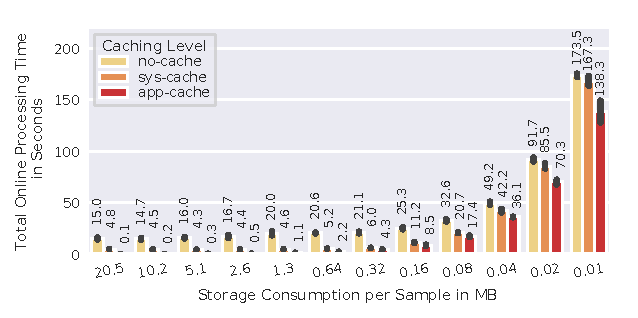
\includegraphics[width=0.47\textwidth]{figures/misc/synthetic-dataset-all-caches}
    \vspace{-14pt}
    \caption{{\color{diff}Online processing time for different caching levels and sample sizes of a synthetic 15\:GB dataset.}}
    \label{fig:synthetic-dataset-cached-general}
\end{figure}
%\vspace{-0.5cm}
}

{\color{diff2}

We investigate this observation by profiling synthetic \texttt{float32} datasets with different sample sizes with both system- and application-level caching (Fig.~\ref{fig:synthetic-dataset-cached-general}).
At the lower end of storage consumption, starting with 0.16\:MB per sample, reading smaller samples takes increasingly longer.
The smaller the sample size, the more processing time the deserialization takes, which lessens the final throughput of the cached dataset.
At 0.04\:MB and lower, the processing time when data is cached in memory (\texttt{sys-cache}) is comparable to the case where data is on storage (\texttt{no-cache}), nullifying the effects of caching.

}

{\color{diff}

Our real-world experiments show the same behaviour.
The storage consumption per sample for MP3 is 0.08\:MB at the \texttt{spectrogram\\-encoded} strategy, while having a relative throughput increase of $1.6\times$ (Fig.~\ref{fig:caching-mp3}) with caching.
Meanwhile, the FLAC pipeline has a storage consumption of 0.4\:MB per sample with the same strategy and increases its throughput by $4.2\times$ (Fig.~\ref{fig:caching-flac}) with caching.
The NILM pipeline shows almost no increase in throughput ($1.1\times$) over multiple epochs (Fig.~\ref{fig:caching-nilm}) as the sample size is only 0.012\:MB.

While this is interesting, system-level caching via the page cache is somewhat unsatisfactory, since one wants to cache the tensor data and not be bottlenecked by the deserialization.
The TensorFlow function \texttt{tf.data.Dataset.cache} caches the deserialized tensors in memory, avoiding deserialization overheads.
This leads us to our fourth observation.

%\vspace{-0.1cm}
\begin{table}[h]
\scalebox{0.8}{
\begin{tabular}{l|r|r|r}
\textbf{Pipeline} & \textbf{System-level} & \textbf{Application-level} & \textbf{Sample Size} \\ \hline
CV2-JPG           & $3.3\times$ & $15.2\times$ & 1.18\:MB \\ \hline
CV2-PNG           & $3.5\times$ & $14.5\times$ & 1.18\:MB \\ \hline
FLAC              & $4.2\times$ & $8.0\times$ & 0.41\:MB \\ \hline
MP3               & $1.6\times$ & $2.2\times$ & 0.08\:MB \\ \hline
NILM              & $1.1\times$ & $1.4\times$ & 0.01\:MB \\
\end{tabular}
}
\caption{{\color{diff}Throughput increase for different caching level compared to no caching of of each pipeline's last strategy.}}
\label{tab:throughput-caching-levels}
\end{table}
\vspace{-0.7cm}

\textbf{(4) Application-level caching is more efficient than system-level caching, but is still affected by the storage consumption per sample. }

}

{\color{diff2}

To understand how application-level caching affects the performance, we profiled all pipeline's respective last strategies, as well as our synthetic 15\:GB datasets again with application-level caching.
The results of the synthetic datasets in Fig.~\ref{fig:synthetic-dataset-cached-general} (\texttt{app-cache}) show that application-level caching is faster, but there is the same pattern of increasing processing time with a smaller sample size.
The online processing time with application-level caching consists solely of reading the samples from memory.
We can calculate the time spent on deserialization by subtracting the \texttt{app-cache} time from \texttt{sys-cache} time.
By dividing with the \texttt{sys-cache} time, we can get the percentage of the time spent on deserialization.
For the sample sizes 20.5\:MB to 5.1\:MB we spend 94-98\% time on deserialization ($\frac{4.8-0.1}{4.8}$), compared to 14-18\% for 0.08\:MB to 0.01\:MB ($\frac{167.3-138.3}{167.3}$).
Hence, the largest relative gains with application-level caching can be achieved with large sample sizes.

Our real-world pipelines have shown a similar throughput improvement compared to system-level caching when the dataset fits into memory (Tab.~\ref{tab:throughput-caching-levels}).
The decline in throughput improvement with both caching levels is directly correlated with a smaller sample size.
The last strategies of the CV and NLP pipelines failed to run with application-level caching as the dataset did not fit into the cache (cf. Sec.~\ref{ssec:caching} \textbf{(1)}).

}
















{\color{diff}

\subsection{Compression}
\label{ssec:compression}

Storage consumption has shown to be an important factor for throughput.
Compression adds a new possibility to decrease storage consumption at the cost of an offline compression step and an online decompression step.
For compression to provide a benefit, the gains of decreased data size must outweigh the computational overheads.
A common metric to evaluate compression on storage consumption is the \textit{space saving} percentage.
For example, if the size did not change after compression, the space saving is 0\%.
When it changes from originally 5\:GB to 1\:GB, the space saving is 80\%.
We omitted the \texttt{unprocessed} strategy for all pipelines because accessing single files is bound by the random access performance of the storage (cf. Sec.~\ref{ssec:storage-versus-throughput} \textbf{(1)}) and compression does not help with this issue.
\begin{figure}
    \begin{subfigure}[c]{0.26\textwidth}
        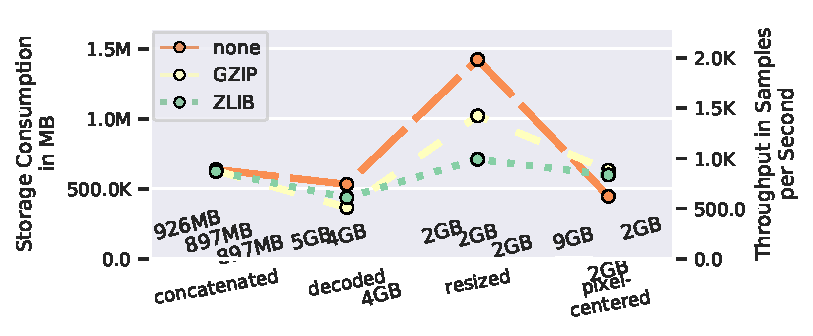
\includegraphics[width=\textwidth]{figures/imagenet-pipeline/compressed-storage-vs-throughput.pdf}
        \vspace{-18pt}
        \caption{CV\footnotemark[1]}
        \label{fig:compressed-storage-vs-throughput-cv}
    \end{subfigure}
    \begin{subfigure}[c]{0.21\textwidth}
        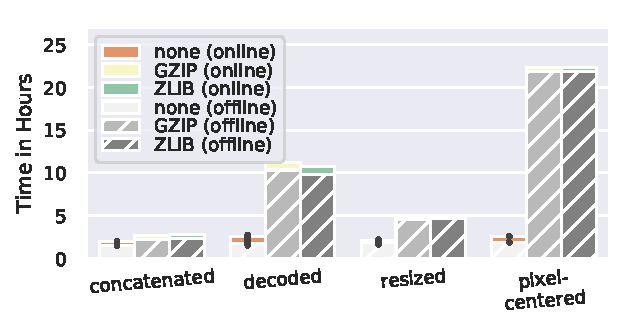
\includegraphics[width=\textwidth]{figures/imagenet-pipeline/compression-processing-time-split.pdf}
        \vspace{-18pt}
        \caption{CV\footnotemark[1]}
        \label{fig:compressed-processing-time-cv}
    \end{subfigure}
    \begin{subfigure}[c]{0.26\textwidth}
        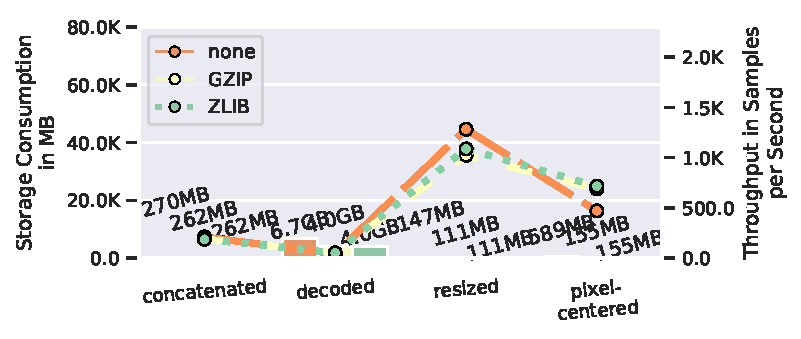
\includegraphics[width=\textwidth]{figures/cubeplusplus-jpg-pipeline/compressed-storage-vs-throughput.pdf}
        \vspace{-18pt}
        \caption{CV2-JPG}
        \label{fig:compressed-storage-vs-throughput-cv2-jpg}
    \end{subfigure}
    \begin{subfigure}[c]{0.21\textwidth}
        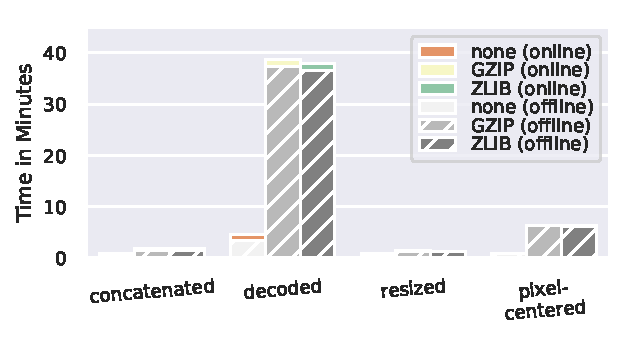
\includegraphics[width=\textwidth]{figures/cubeplusplus-jpg-pipeline/compression-processing-time-split.pdf}
        \vspace{-18pt}
        \caption{CV2-JPG}
        \label{fig:compressed-processing-time-cv2-jpg}
    \end{subfigure}
    \begin{subfigure}[c]{0.26\textwidth}
        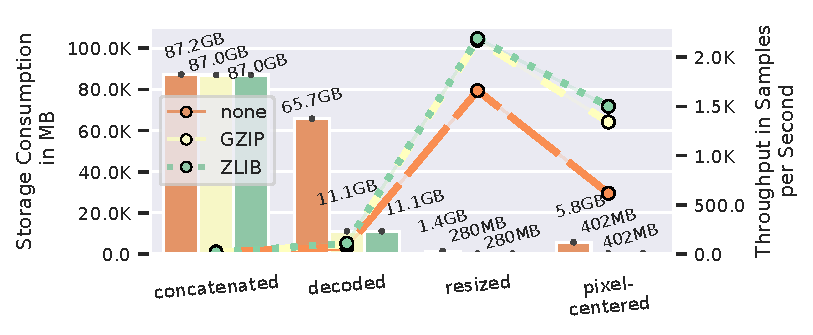
\includegraphics[width=\textwidth]{figures/cubeplusplus-png-pipeline/compressed-storage-vs-throughput.pdf}
        \vspace{-18pt}
        \caption{CV2-PNG}
        \label{fig:compressed-storage-vs-throughput-cv2-png}
    \end{subfigure}
    \begin{subfigure}[c]{0.21\textwidth}
        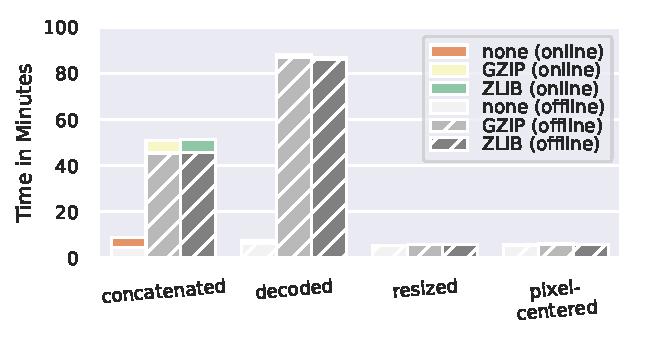
\includegraphics[width=\textwidth]{figures/cubeplusplus-png-pipeline/compression-processing-time-split.pdf}
        \vspace{-18pt}
        \caption{CV2-PNG}
        \label{fig:compressed-processing-time-cv2-png}
    \end{subfigure}
    \begin{subfigure}[c]{0.26\textwidth}
        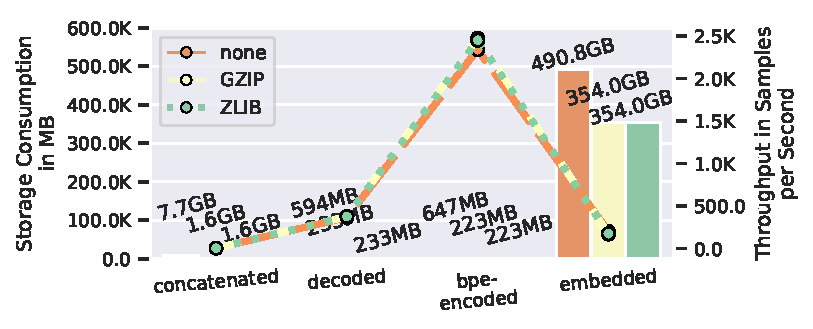
\includegraphics[width=\textwidth]{figures/openwebtext-pipeline/compressed-storage-vs-throughput.pdf}
        \vspace{-18pt}
        \caption{NLP}
        \label{fig:compressed-storage-vs-throughput-nlp}
    \end{subfigure}
    \begin{subfigure}[c]{0.21\textwidth}
        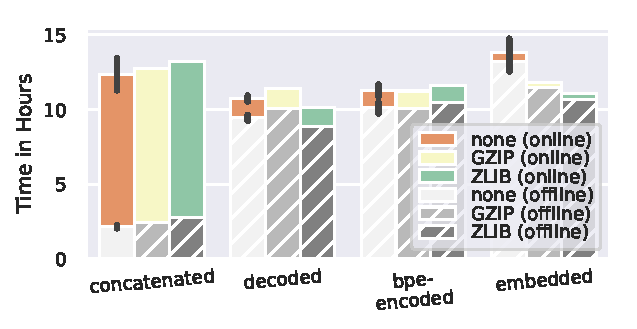
\includegraphics[width=\textwidth]{figures/openwebtext-pipeline/compression-processing-time-split.pdf}
        \vspace{-18pt}
        \caption{NLP}
        \label{fig:compressed-processing-time-nlp}
    \end{subfigure}
    \begin{subfigure}[c]{0.26\textwidth}
        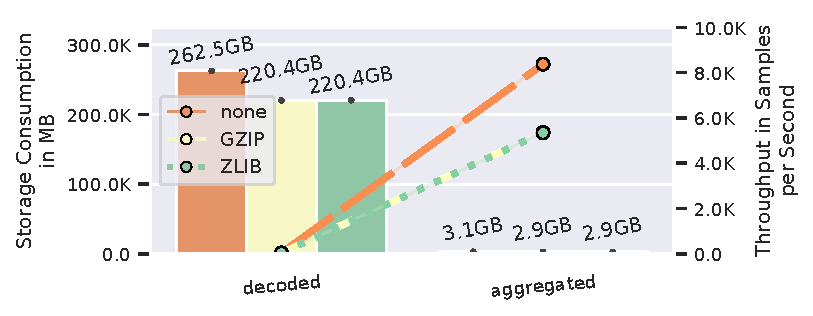
\includegraphics[width=\textwidth]{figures/cream-pipeline/compressed-storage-vs-throughput.pdf}
        \vspace{-18pt}
        \caption{NILM}
        \label{fig:compressed-storage-vs-throughput-nilm}
    \end{subfigure}
    \begin{subfigure}[c]{0.21\textwidth}
        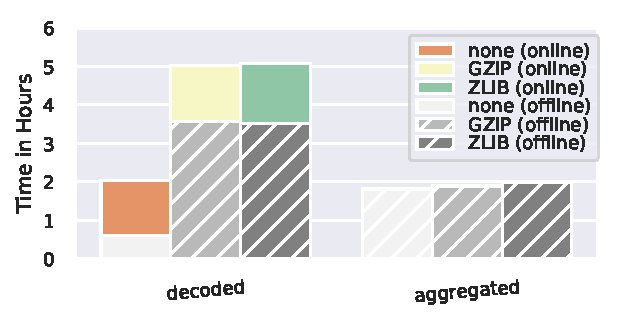
\includegraphics[width=\textwidth]{figures/cream-pipeline/compression-processing-time-split.pdf}
        \vspace{-18pt}
        \caption{NILM}
        \label{fig:compressed-processing-time-nilm}
    \end{subfigure}
    \begin{subfigure}[c]{0.26\textwidth}
        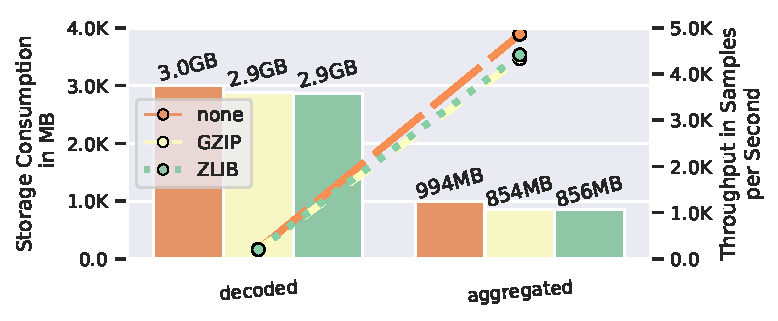
\includegraphics[width=\textwidth]{figures/commonvoice-pipeline/compressed-storage-vs-throughput.pdf}
        \vspace{-18pt}
        \caption{MP3}
        \label{fig:compressed-storage-vs-throughput-mp3}
    \end{subfigure}
        \begin{subfigure}[c]{0.21\textwidth}
        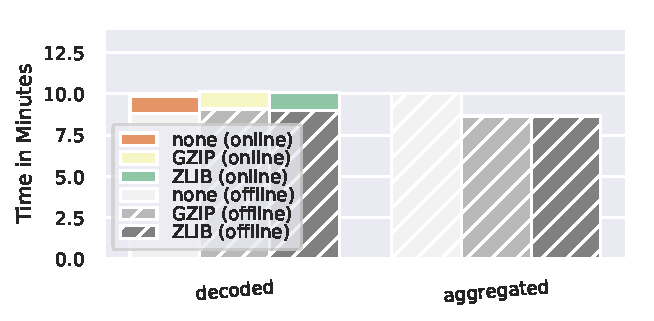
\includegraphics[width=\textwidth]{figures/commonvoice-pipeline/compression-processing-time-split.pdf}
        \vspace{-18pt}
        \caption{MP3}
        \label{fig:compressed-processing-time-mp3}
    \end{subfigure}    
    \begin{subfigure}[c]{0.26\textwidth}
        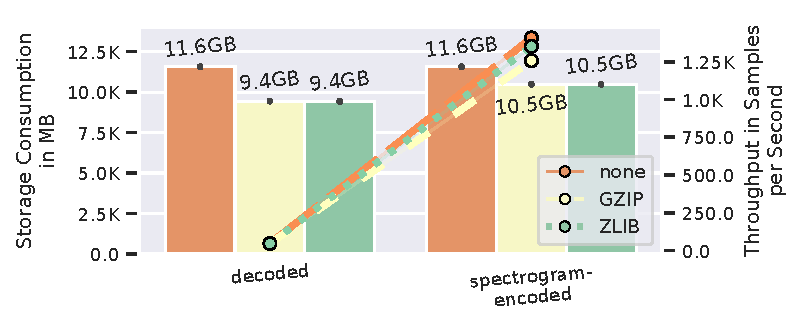
\includegraphics[width=\textwidth]{figures/librispeech-pipeline/compressed-storage-vs-throughput.pdf}
        \vspace{-18pt}
        \caption{FLAC}
        \label{fig:compressed-storage-vs-throughput-flac}
    \end{subfigure}
    \begin{subfigure}[c]{0.21\textwidth}
        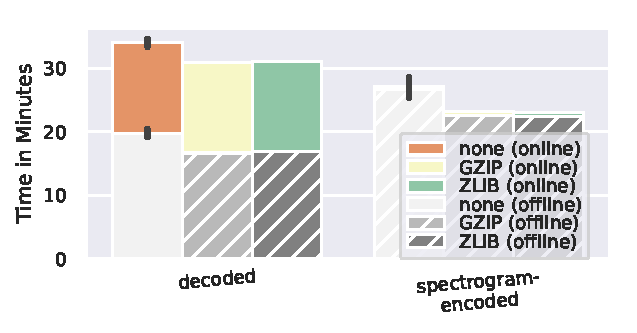
\includegraphics[width=\textwidth]{figures/librispeech-pipeline/compression-processing-time-split.pdf}
        \vspace{-18pt}
        \caption{FLAC}
        \label{fig:compressed-processing-time-flac}
    \end{subfigure}
    \vspace{-0.3cm}
    \caption{{\color{diff}Left column: Storage consumption compared to $T_4$ throughput (dotted lines) with compression. Right column: Offline (grey hatched bars) and online processing time (colored) with compression.}}
    \label{fig:compression-results}
\end{figure}
\footnotetext[1]{Unfortunately, after one full run with each compression library (GZIP, ZLIB) for each strategy of the CV pipeline, our CEPH storage system was reconfigured which led to non-comparable results of the respective repeat runs. Hence, for these specific experiments, we only report results of one run (instead of the average of five runs, as in all other experiments).}
The results of our compression experiments are shown in Fig.~\ref{fig:compression-results}.
We make the following observations:

\textbf{(1) High space savings do not guarantee improved throughput.}

Space saving affects the throughput positively for some, but not all strategies.
All CV-based pipelines had an increase in throughput with compression between $1.6\times$ and $2.4\times$ at \texttt{pixel-centered} where space saving is between 73\% and 93\% (Fig.~\ref{fig:compressed-storage-vs-throughput-cv},~\ref{fig:compressed-storage-vs-throughput-cv2-jpg},~\ref{fig:compressed-storage-vs-throughput-cv2-png}).
In this case, the faster read time in total was beneficial compared to the cost of the additional decompression step.

In contrast, the strategies of the NLP pipeline have a space saving between 28\% and 80\%, but none of them had a throughput increase (Fig.~\ref{fig:compressed-storage-vs-throughput-nlp}).
The reason for that is that every strategy was bound by a computationally expensive CPU step except the last strategy \texttt{embedded}.
At \texttt{embedded}, the dataset is only read from disk and deserialized, but the space saving of 28\% was not enough to benefit the total throughput.

The same effect becomes visible when comparing the strategies \texttt{decoded} and \texttt{resized} between the CV2-PNG and CV2-JPG pipelines (Fig.~\ref{fig:compressed-storage-vs-throughput-cv2-jpg},~\ref{fig:compressed-storage-vs-throughput-cv2-png}).
The only difference between the pipelines is the encoding of the images, with JPG being a lossy storage format, while PNG is lossless.
The CV2-PNG pipeline has a better space saving with compression with the \texttt{decoded} strategy (83\%) compared to CV2-JPG (41\%).
This results in a throughput increase by $1.5\times$ for CV2-PNG compared to the 89\% throughput deterioration at CV2-JPG.
The \texttt{resized} strategy with the PNG images has a space saving of 81\% and improves the throughput by $1.3\times$, while JPG only saves 24\% of space and reduces the throughput to 96\%.
The compression artifacts introduced by the lossy JPG encoding affect the space saving of both GZIP and ZLIB negatively.

All the other pipelines, NILM, MP3 and FLAC, slow down with compression and have a varying space saving between 0.3-41.2\% (Fig.~\ref{fig:compressed-storage-vs-throughput-nilm},~\ref{fig:compressed-storage-vs-throughput-mp3},~\ref{fig:compressed-storage-vs-throughput-flac}).
When comparing the different compression types, ZLIB was slightly faster and had a comparable space saving to GZIP, except for NLP's \texttt{bpe-encoded}, where it was slightly slower compared to GZIP.

\textbf{(2) Offline compression and write time can be volatile. }

When compressing a dataset, the processing time is increased by the compression algorithm, and decreased by the lower write time due to lower storage consumption.
The balance between these steps is not predictable from our observations, as the CV2-PNG pipeline shows (Fig.~\ref{fig:compressed-processing-time-cv2-png}). 
With the \texttt{concatenated} strategy and a space saving of only 0.3\%, it takes $9.6\times$ longer to save the dataset to storage.
The strategy \texttt{decoded} has a space saving of 83\% and takes $13.5\times$ longer for offline processing.
The next strategies, \texttt{resized} and \texttt{pixel-centered}, have a space saving of 80\%-93\% and only take 1.08-1.1$\times$ longer.
Compared to a slightly worse space saving of 74\% with the \texttt{pixel-centered} strategy at the CV2-JPG pipeline (Fig.~\ref{fig:compressed-processing-time-cv2-jpg}), the offline processing time is increased by $6.1\times$. 

Generally, we see examples of a high space saving and no effective increase in offline processing time in NLP (Fig.~\ref{fig:compressed-processing-time-nlp}), a low space saving with a higher offline processing time in NILM (Fig.~\ref{fig:compressed-processing-time-nilm}) and CV2-PNG \texttt{concatenated} (Fig.~\ref{fig:compressed-processing-time-cv2-png}), and low space saving with no effective increase in offline processing time in MP3 (Fig.~\ref{fig:compressed-processing-time-mp3}), FLAC (Fig.~\ref{fig:compressed-processing-time-flac}), and CV \texttt{concatenated} and \texttt{resized} (Fig.~\ref{fig:compressed-processing-time-cv}). Space saving does not seem to be a good predictor at how the compression will affect the offline processing time.

}



{\color{diff}

\subsection{Parallelization Capabilities}
\label{ssec:parallelization-capabilities}

\vspace{-0.45cm}
\begin{figure}[h]
    \centering
    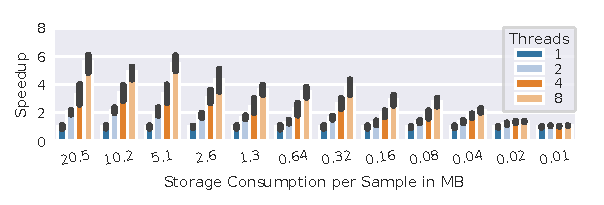
\includegraphics[width=0.47\textwidth]{figures/misc/artificial-dataset-float-multithreaded}
    \vspace{-15pt}
    \caption{{\color{diff}Reading a synthetic 15\:GB dataset with different sample sizes to compare multi-threaded scalability.}}
    \label{fig:synthetic-dataset-speedup}
\end{figure}
\vspace{-0.2cm}


\begin{figure}
    \begin{subfigure}[c]{0.22\textwidth}
        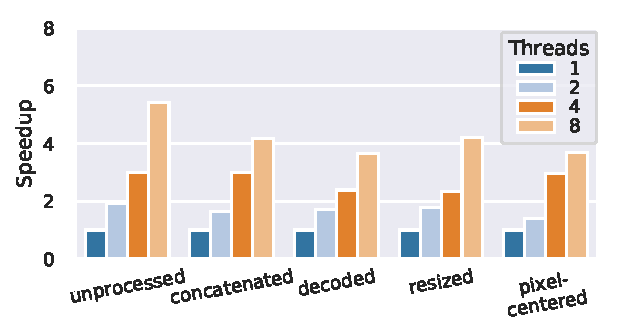
\includegraphics[width=\textwidth]{figures/imagenet-pipeline/speedup-8000-samples-epoch-0.pdf}
        \vspace{-18pt}
        \caption{CV \texttt{no-cache}}
        \label{fig:speedup-cv}
    \end{subfigure}
    \begin{subfigure}[c]{0.22\textwidth}
        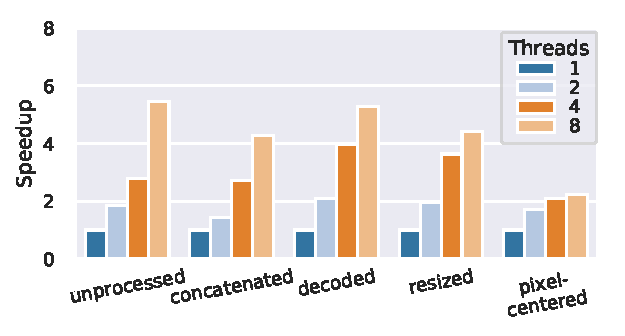
\includegraphics[width=\textwidth]{figures/imagenet-pipeline/speedup-8000-samples-epoch-1.pdf}
        \vspace{-18pt}
        \caption{CV \texttt{sys-cache}}
        \label{fig:speedup-epochs-cv}
    \end{subfigure}
    \begin{subfigure}[c]{0.22\textwidth}
        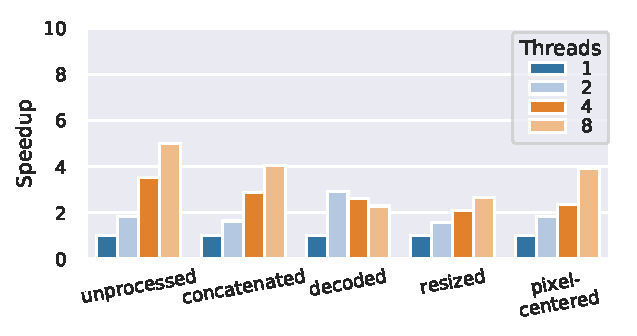
\includegraphics[width=\textwidth]{figures/cubeplusplus-jpg-pipeline/speedup-4890-samples-epoch-0.pdf}
        \vspace{-18pt}
        \caption{CV2-JPG \texttt{no-cache}}
        \label{fig:speedup-cv2-jpg}
    \end{subfigure}
    \begin{subfigure}[c]{0.22\textwidth}
        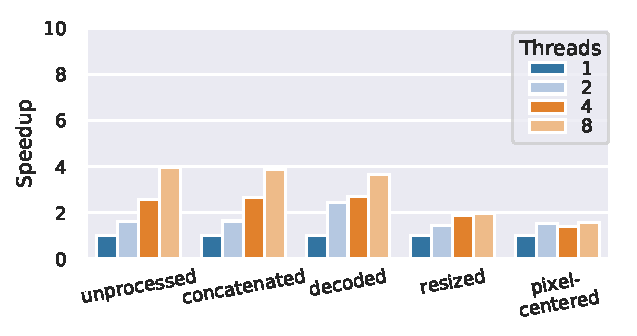
\includegraphics[width=\textwidth]{figures/cubeplusplus-jpg-pipeline/speedup-4890-samples-epoch-1.pdf}
        \vspace{-18pt}
        \caption{CV2-JPG \texttt{sys-cache}}
        \label{fig:fig:speedup-epochs-cv2-jpg}
    \end{subfigure}
    \begin{subfigure}[c]{0.22\textwidth}
        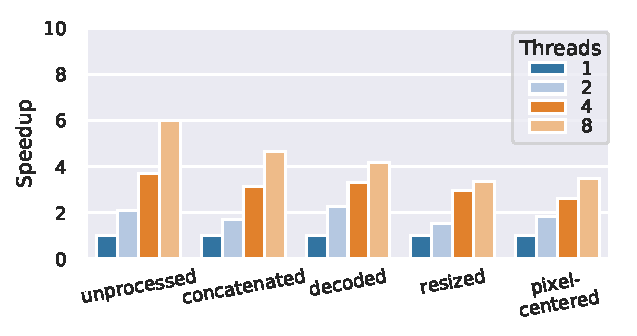
\includegraphics[width=\textwidth]{figures/cubeplusplus-png-pipeline/speedup-4890-samples-epoch-0.pdf}
        \vspace{-18pt}
        \caption{CV2-PNG \texttt{no-cache}}
        \label{fig:speedup-cv2-png}
    \end{subfigure}
    \begin{subfigure}[c]{0.22\textwidth}
        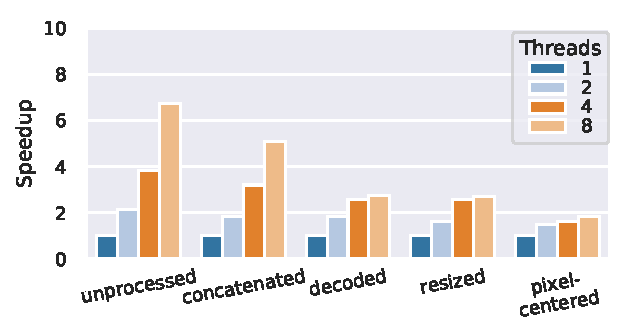
\includegraphics[width=\textwidth]{figures/cubeplusplus-png-pipeline/speedup-4890-samples-epoch-1.pdf}
        \vspace{-18pt}
        \caption{CV2-PNG \texttt{sys-cache}}
        \label{fig:speedup-epochs-cv2-png}
    \end{subfigure}
    \begin{subfigure}[c]{0.22\textwidth}
        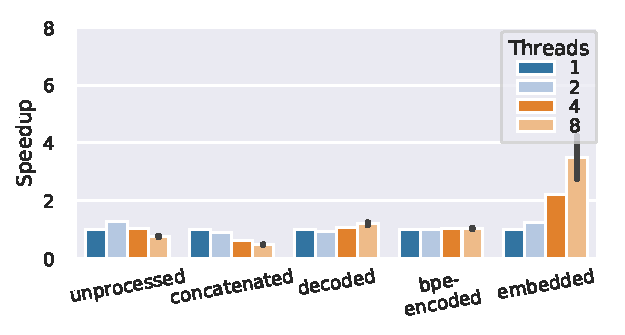
\includegraphics[width=\textwidth]{figures/openwebtext-pipeline/speedup-8000-samples-epoch-0.pdf}
        \vspace{-18pt}
        \caption{NLP \texttt{no-cache}}
        \label{fig:speedup-nlp}
    \end{subfigure}
    \begin{subfigure}[c]{0.22\textwidth}
        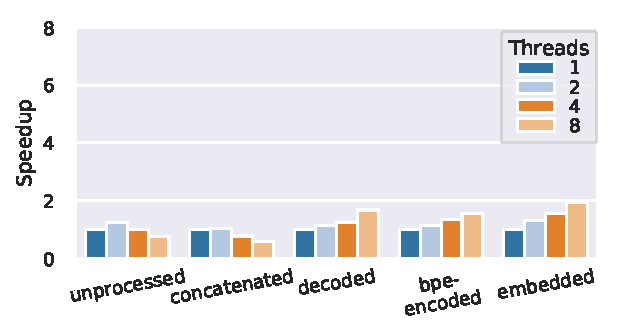
\includegraphics[width=\textwidth]{figures/openwebtext-pipeline/speedup-8000-samples-epoch-1.pdf}
        \vspace{-18pt}
        \caption{NLP \texttt{sys-cache}}
        \label{fig:speedup-epochs-nlp}
    \end{subfigure}
    \begin{subfigure}[c]{0.22\textwidth}
        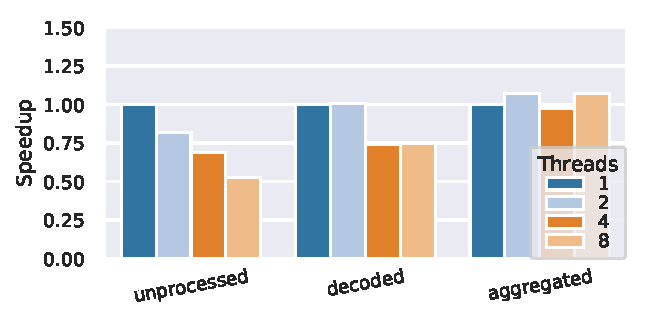
\includegraphics[width=\textwidth]{figures/cream-pipeline/speedup-8000-samples-epoch-0.pdf}
        \vspace{-18pt}
        \caption{NILM \texttt{no-cache}}
        \label{fig:speedup-nilm}
    \end{subfigure}
    \begin{subfigure}[c]{0.22\textwidth}
        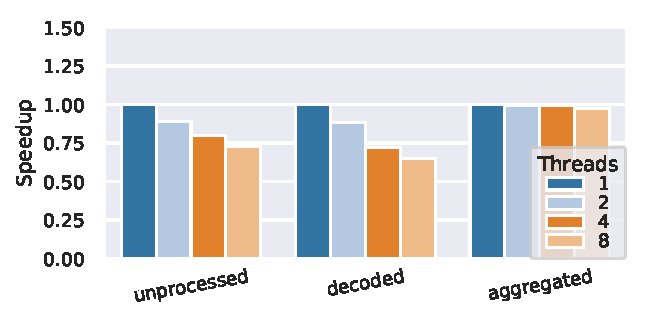
\includegraphics[width=\textwidth]{figures/cream-pipeline/speedup-8000-samples-epoch-1.pdf}
        \vspace{-18pt}
        \caption{NILM \texttt{sys-cache}}
        \label{fig:speedup-epochs-nilm}
    \end{subfigure}
    \begin{subfigure}[c]{0.22\textwidth}
        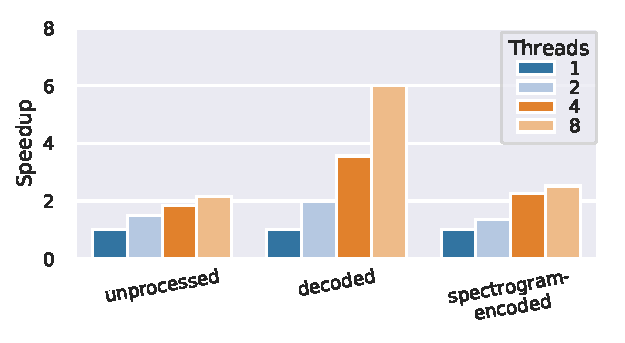
\includegraphics[width=\textwidth]{figures/commonvoice-pipeline/speedup-8000-samples-epoch-0.pdf}
        \vspace{-18pt}
        \caption{MP3 \texttt{no-cache}}
        \label{fig:speedup-mp3}
    \end{subfigure}
        \begin{subfigure}[c]{0.22\textwidth}
        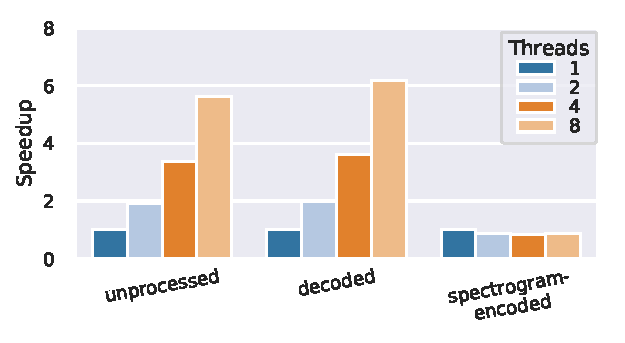
\includegraphics[width=\textwidth]{figures/commonvoice-pipeline/speedup-8000-samples-epoch-1.pdf}
        \vspace{-18pt}
        \caption{MP3 \texttt{sys-cache}}
        \label{fig:speedup-epochs-mp3}
    \end{subfigure}
    \begin{subfigure}[c]{0.22\textwidth}
        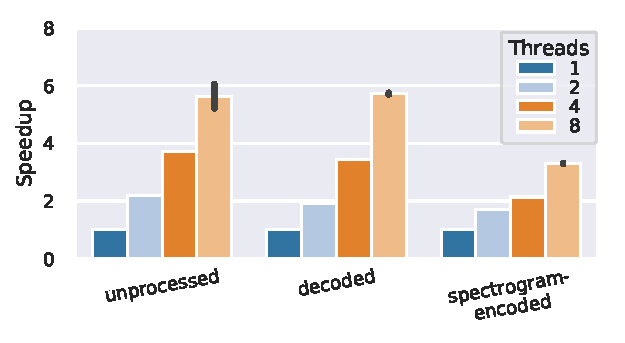
\includegraphics[width=\textwidth]{figures/librispeech-pipeline/speedup-8000-samples-epoch-0.pdf}
        \vspace{-18pt}
        \caption{FLAC \texttt{no-cache}}
        \label{fig:speedup-flac}
    \end{subfigure}
    \begin{subfigure}[c]{0.22\textwidth}
        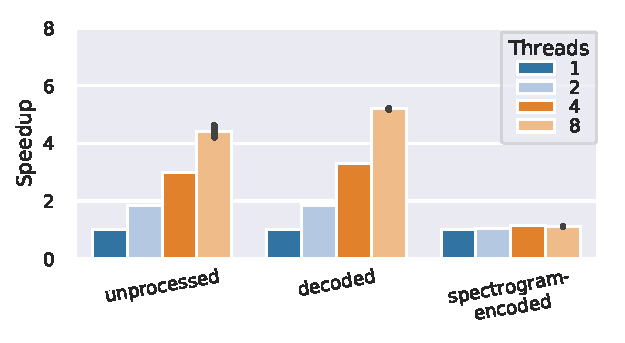
\includegraphics[width=\textwidth]{figures/librispeech-pipeline/speedup-8000-samples-epoch-1.pdf}
        \vspace{-18pt}
        \caption{FLAC \texttt{sys-cache}}
        \label{fig:speedup-epochs-flac}
    \end{subfigure}
    \vspace{-0.3cm}
    \caption{{\color{diff}Speedup at 8000 samples. Left column: No caching. Right column: System-level caching.}}
    \label{fig:speedup}
\end{figure}


We analyzed the parallelization capabilities of each pipeline under multi-threading, as this is one of the best practice recommendations to speed up data pipelines and remove I/O bottlenecks~\cite{tfdatabestpractice2020}.
We compared the speedup of each strategy by running it with 1, 2, 4, and 8 threads over two epochs with system-level caching enabled (Fig.~\ref{fig:speedup}).
The profiling was done with a fraction of the dataset (up to 8000 samples) so that the second epoch could be fully cached for each pipeline to compare the speedup with system-level caching.
We make the following observations:

\textbf{(1) A small storage consumption per sample hinders multi-threaded performance.}
We know from the previous Sections~\ref{ssec:storage-versus-throughput} and \ref{ssec:caching} that a small storage consumption per sample affects the online preprocessing time negatively.
However, how does it affect multi-threaded execution?
To analyze this, we reused the same synthetic 15\:GB \texttt{float32} dataset with different sample sizes to compare their multi-threaded read and deserialization time.
The results in Fig.~\ref{fig:synthetic-dataset-speedup} show a similar trend as before, with a speedup of close to 1$\times$ for the 0.01\:MB sample sizes.
This means that processing small samples with a single thread takes equally long as with eight threads.
}
{\color{diff2}
We traced the issue down to an increased amount of context switches with smaller sample sizes (100,000 per second at 0.01\:MB compared to 5,000 per second for 20.5\:MB).
Additionaly, as we extracted from the trace log, every thread only processes a single sample at a time and is finished faster with smaller sample sizes before being scheduled again.
Scheduling a thread to process a new sample induces so much overhead that multi-threading can not be effective at small sample sizes.
}

{\color{diff}

A good example from our real-world pipelines is NILM (Fig.~\ref{fig:speedup-nilm}) at the \texttt{aggregated} strategy, which has no effective speedup due to a sample size of 0.01\:MB.
Even when reading the dataset from memory (Fig.~\ref{fig:speedup-epochs-nilm}), there is virtually no change in speedup.
Every last strategy from each pipeline has as slightly worse speedup when reading from memory (\texttt{sys-cache}) than when reading from storage (\texttt{no-cache}) (Fig.~\ref{fig:speedup}).
The reason for this is that memory provides a higher bandwidth, so reading data is fast, even with a single thread.
Therefore, the effect of context switches is highlighted even more compared to the case where the slower network read speeds affects the total processing time additionally.

\newpage
\textbf{(2) Inefficient preprocessing can reduce multi-threading scalability. }

While most of the scaling issues like \texttt{bpe-encoding} in NLP can be explained with a small sample size (0.003\:MB), we also observed slowdowns (speedup $< 1.0$), which have a different root cause.
This happens with the first two strategies of NILM (Fig.~\ref{fig:speedup-nilm}, 0.15\:MB and 0.98\:MB) and NLP (Fig.~\ref{fig:speedup-nlp}, 0.04MB), which are not alleviated by reading from memory (Fig.~\ref{fig:speedup-epochs-nilm}, ~\ref{fig:speedup-epochs-nlp}, respectively).
This points to a processing issue.
One thing that both \texttt{unprocessed}, \texttt{concatenated} (NLP) and \texttt{decoded} (NILM) have in common, is that they are using external Python libraries like NumPy and newspaper wrapped in a \texttt{tf.py\_function}, while all the other preprocessing steps are provided by the TensorFlow library.

}

{\color{diff2}
\vspace{-0.3cm}
\begin{figure}[h]
    \begin{subfigure}[c]{0.23\textwidth}
        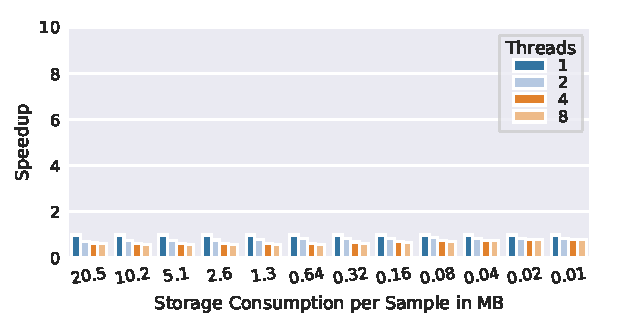
\includegraphics[width=\textwidth]{figures/misc/artificial-dataset-speedup-np-raw.pdf}
        \vspace{-18pt}
        \caption{NumPy RMS}
        \label{fig:synthetic-dataset-processing-np}
    \end{subfigure}
    \begin{subfigure}[c]{0.23\textwidth}
        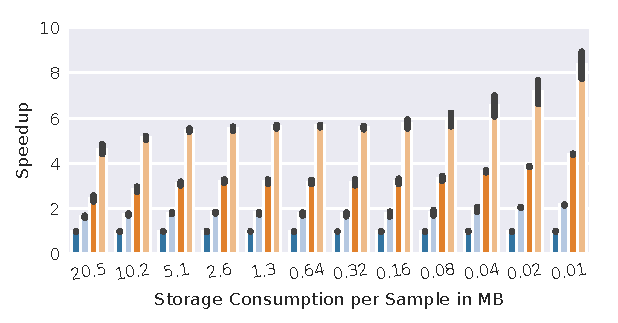
\includegraphics[width=\textwidth]{figures/misc/artificial-dataset-speedup-tf-raw.pdf}
        \vspace{-18pt}
        \caption{TensorFlow RMS}
        \label{fig:synthetic-dataset-processing-tf}
    \end{subfigure}
    \vspace*{-0.3cm}
    \caption{{\color{diff2}Speedup of applying RMS to a synthetic 15\:GB dataset with different sample sizes implemented in NumPy and TensorFlow. }}
    \label{fig:synthetic-dataset-tf-vs-np}
\end{figure}
\vspace{-0.3cm}

To test how external libraries affect the throughput, we created a new preprocessing step which applies the root-mean-square (RMS) function with a period of 500 over the entire sample, leaning on a similar computation from the NILM pipeline.
We implemented this step both with NumPy and TensorFlow, and we profile our synthetic datasets with steps applied online individually.
The results in Fig.\ref{fig:synthetic-dataset-tf-vs-np} show that the NumPy implementation has the same slowdown as NILM and NLP for all sample sizes, whereas the TensorFlow implementation shows a speedup between 4-8$\times$ for eight threads.
However, while the NumPy implementation does not scale, it is still 2.9$\times$ faster with a single-threaded processing time of 650 seconds compared to TensorFlow's 1905 seconds with eight threads at the 20.5\:MB sample size.
In other words, it pays off to use the less scalable but more efficient implementation in NumPy instead of the native implementation in TensorFlow.

}

{\color{diff}

\textbf{(3) Random file access performance can affect the speedup. }
We have already discussed the impact of concatenation in Sec.~\ref{ssec:storage-versus-throughput} \textbf{(1)} and how random file access can hinder achieving high throughput and bandwidth utilization.
By running the multi-threading experiments with system-level caching enabled, we can isolate the effect of random file access on speedup.
For example, the \texttt{unprocessed} strategy of the MP3 pipeline (Fig.~\ref{fig:speedup-mp3}) has a speedup of $2\times$ when reading from storage with eight threads, versus a speedup of $6\times$ when reading from memory (Fig.~\ref{fig:speedup-epochs-mp3}).
This shows that decoding does in fact scale well.
The same effect changes the speedup of the FLAC pipeline from 4$\times$ (Fig.~\ref{fig:speedup-flac}) to 6$\times$ with eight threads (Fig.~\ref{fig:speedup-epochs-flac}).

}

\subsection{Shuffling}
\label{ssec:shuffling}

A common technique in DL is to change the order of the dataset in every epoch, so the optimizers do not see the same gradients in mini-batches.
There are a few different approaches to shuffling the dataset, which include sampling from the dataset \textit{with-} or \textit{without replacement}~\cite{de2020random,haochen2019random,yun2021singleshuffle}.
Irrespective of which algorithm is used to modify the order of the dataset, it is a very memory-intensive problem, as the entire dataset has to be loaded into RAM.
One solution is to create a buffer that fits into the memory and use a \textit{with-replacement} sampling strategy to iterate over the entire dataset in a pseudo-random fashion~\cite{tfdatasetapishuffle}, similar to reservoir sampling~\cite{10.1145/3147.3165}.

We implemented and profiled this approach with multiple sample counts, which confirms the naive assumption that the \textit{per-sample} processing time for shuffling is constant.
That means that shuffling has a linear relation to storage consumption and is not specific to a pipeline or dataset.
The difference in per-sample processing time between shuffling and not shuffling for each sample size is $(\pm0.5)$ 9.6ms on average.
An additional characteristic is that the initial call to allocate a buffer is amortized with a bigger sample size, which manifests itself in the increasingly faster per-sample time with incremented sample sizes. 

PRESTO's profiling can help to find the optimal place in the pipeline where shuffling should be applied.
As the storage consumption of a strategy does not affect the runtime of shuffling, we do not recommend making shuffling part of the strategy selection.
However, once a strategy is determined, we suggest to shuffle after the online pipeline step that yields the smallest data size.
If we consider a fixed-size buffer for shuffling, the highest number of samples can be fit into the buffer when the size of the data sample is smallest.
The higher the number of samples in the buffer, the higher the entropy; this, in turn, leads to a better approximation of the ``true'' gradient~\cite{ruder2016overview,kingma2014adam}.

{\color{diff}

\subsection{Modifying the Pipeline}
\label{ssec:modifying-pipeline}

We added an additional preprocessing step to the CV pipeline to showcase how the trade-offs can shift in an already profiled pipeline.
We decided on adding a step that converts images from RBG to greyscale because this is a common preprocessing step that affects the storage consumption and is not obviously compute intensive.
To evaluate how an additional step will affect the pipeline performance, we profiled two setups: before and after the \texttt{pixel-centered} strategy.

}

\vspace{-0.2cm}
\begin{figure}[h]
    \begin{subfigure}[c]{0.23\textwidth}
        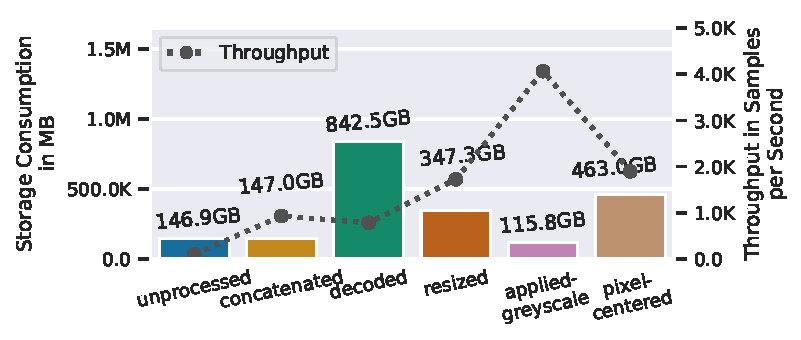
\includegraphics[width=\textwidth]{figures/imagenet-pipeline/storage-vs-throughput-gs-after-resize.pdf}
        \vspace{-18pt}
        \caption{{\color{diff}Before Pixel Centering}}
        \label{fig:ss-vs-thr-gs-before-pc}
    \end{subfigure}
    \begin{subfigure}[c]{0.23\textwidth}
        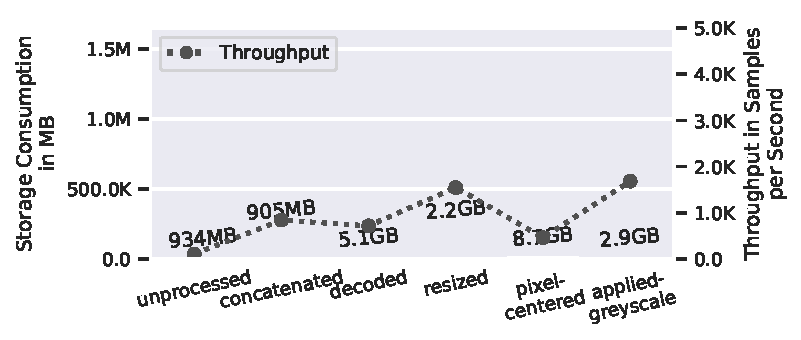
\includegraphics[width=\textwidth]{figures/imagenet-pipeline/storage-vs-throughput-gs-after-pc.pdf}
        \vspace{-18pt}
        \caption{{\color{diff}After Pixel Centering}}
        \label{fig:ss-vs-thr-gs-after-pc}
    \end{subfigure}
    \vspace{-10pt}
    \caption{{\color{diff}Storage consumption (left y-axis) and throughput (right y-axis, dotted line) comparison of adding a greyscale transformation before and after the pixel centering.}}
    \label{fig:imagenet-greyscale-comparison}
\end{figure}
\vspace{-0.2cm}

{\color{diff3}

Before discussing the results, we explain the characteristics of the new \texttt{applied-greyscale} strategy and compare it to \texttt{resized}.
Converting a 3-channel image to greyscale should decrease the storage consumption by 3$\times$, because we only need a single channel with the same datatype.
The \texttt{resized} strategy reduces the size by 2.4$\times$ for the CV dataset, which is dependent on the average image resolution.
Adding greyscaling will also affect the throughput of \texttt{pixel-centered} as the final storage consumption will be reduced as well.

The results in Fig.~\ref{fig:imagenet-greyscale-comparison} show the effect of the additional greyscale step on the storage consumption and throughput. 
First of all, applying the greyscale step before the \texttt{pixel-centered} strategy increases the maximum throughput of the pipeline by 2.8$\times$, from 1513\:SPS with \texttt{resized} (Fig.~\ref{fig:ss-vs-thr-gs-after-pc}) to 4284\:SPS with \texttt{applied-greyscale} (Fig.~\ref{fig:ss-vs-thr-gs-before-pc}).
While the last strategy of both setups performs similary, applying preprocessing steps that reduce the storage consumption consecutively increases the throughput for intermediate strategies.
We additionally evaluated a setup where the resize and greyscale steps are interchanged before the pixel centering, but there was no significant difference in performance to Fig.~\ref{fig:ss-vs-thr-gs-before-pc}.
The second setup with the last strategy \texttt{applied-greyscale} increases the throughput from 534\:SPS at \texttt{pixel-centered} to 1384\:SPS by reducing the data size from 1.4\:TB to 463\:GB.
This supports our observation \textbf{(2)} from Sec.~\ref{ssec:storage-versus-throughput} that steps which reduce storage consumption should be investigated with priority when searching for the best performing.

}
%GSBefore Resize faster: pixel-centered (1530 -> 1780) (no idea why this happens, the data is literally the same, but we can note the improvement compared to CV for pixel-centered, 580sps with 1.4TB)
%-> we can argue the improvement in general for both resized and pixel-centered compared to CV (1813,resized -> 4763,resized + gs-before-resize), (580,pixel-centered -> 1780,pixel-centered + gs-before-resize)
%GSAfter  Resize faster: concatenated (666 -> 1129), decoded (559 -> 694) 


%After Decode: applied-greyscale is faster than resized (1674 -> 2211) (means that the step itself is slightly easier to do for the CPU compared to resize)


%applied-greyscale -> resized: 4763 (makes sense, as app-gs reduces the storage consumption more, therefore its faster)
%resized -> applied-greyscale: 4284 

%O2: The strategy 5 (whatever it is), is still the fastest, and addding an additional preprocessing step actually improved the pipeline performance from (resized original 1813 to 4763 (gs before resize)).